\chapter{Discovering therapeutic targets by genomic profiling of medulloblastoma}
\chaptermark{Discovering therapeutic targets}
\label{ch:target-id}

\begin{objective}
We hypothesize that each medulloblastoma molecular subgroup is characterized by specific genomic alterations, and we aim to identify potential therapeutic targets specific to each molecular subgroup.
\end{objective}

Increased awareness of long-term neurotoxcities of craniospinal irradiation has motivated the de-escalation of radiotherapy by incorporating dose-intensive combination chemotherpay into the treatment regime. In order to eradicate tumour cells, chemotherapy is often intensified to the point where autologous stem cell transplants are required to circumvent patient mortality. Albeit less harmful, chemotherapy is not without neurocognitive and functional consequences for survivors. In one trial, addition of chemotherapy to craniospinal irradiation caused long-term survivors of medulloblastoma to suffer poorer health status \citeref{bull07}. In another trial, patients with medulloblastoma who were treated with chemotherapy alone (vincristine, carboplatin, etoposide, cyclophosphamide, and methotrexate) suffered from declines in neurocognitive function \citeref{rutkowski05}. Perhaps part of the decline could be due to the disease itself; however, even for patients with acute lymphoplastic leukemia, chemotherapy alone (vincristine, methotrexate, prednisone, and antracyclines) can cause reduction in volumes of several neuroanatomic structures of the brain and consequent decline in processing speed, executive function, learning and memory \citeref{zeller13}. Furthermore, chemotherapy causes a myarid of other side-effects; for example, it increases the risk of infection for patients due to suppression of immune system. Chemotherapeutic drugs such as cisplatin can cause permanent hearing loss and peripheral neurotoxicity \citeref{avan15}.

Aside from mounting evidence for long-term adverse effects, combination chemotherapy encountered yet another setback when a prospective trial reported that prolonged dose-intensive chemotherapy (with cisplatin, cyclophosphamide, vincristine, etoposide) for patients with medulloblastoma yielded no improvement in survival (and also resulted in several treatment-associated deaths) \citeref{strother14}. In this trial, the authors treated the patients with 72 weeks of dose-intensity combination therapy, and patients with medulloblastoma showed no improvement in survival (though patients with ependymoma did) \citeref{strother14}. Similar to prior attempts, dose-intensive chemotherapy also caused patient death (toxic mortality) about 10 times more frequently than standard dose  \citeref{dhall08, strother14}. These negative findings indicate that patient survival cannot be improved by simply increasing the dose of chemotherapy, whose arsenal has essentially remained unchanged for decades.

% \citeref{strother14}
% 1/162 died in dose-intensive arm
% 10/166 died in dose-intensive arm
% fisher.test(matrix(c(10, 156, 1, 161), nrow=2))
% p = 0.01, OR = 10.267

To faciliate the discovery of novel therapeutic targets, we sought to identify recurrently dysregulated genes and pathways by analyzing the DNA copy-number profiles of $> 1000$ primary medulloblastoma samples (before radiotherapy and chemotherapy). Genes amplified recurrently across tumours are candidate proto-oncogenes, against which therapeutic agents may be developed. Conversely, genes deleted recurrently are candidate tumour suppressors, and therapeutic interventions may be designed against downstream pathways. Earlier studies aimed at identifying recurrent \gls{cna} or mutations did not identify any highly recurrent focal genetic lesions across medulloblastoma tumours (without classification into subtypes): most focal genetic lesions occur at frequency of less than 10\%, with \gene{MYC} amplification and \gene{PTCH1} mutation representing the most commonly observed events in medulloblastoma \citeref{northcott09, parsons11}. These observations suggest that medulloblastoma is genetically heterogeneous, and classifying medulloblastoma into molecular subgroups may aid the identification of genes and pathways that are recurrently disrupted above the background mutation rate in medulloblastoma.

The four molecular subgroups of medulloblastoma exhibit activation of different transcriptional progrms, which may be shaped by different genetic abnormalities. We therefore stratify our medulloblastoma samples by subgroup status into more homogeneous groups, and we sought to identify recurrent \gls{cns} enriched in or specific to each molecular subgroup. We hypothesize that each medulloblastoma subgroup incurs different genetic events. Accordingly, we hope to reveal dysregulated genes and pathways underlying the tumourigenesis of each subgroup in order to facilitate the development of precise, targeted therapeutic interventions.

% lower dose of cisplatin did not compromise survival among patients with nonmetastatic, near totally resected medulloblastoma \citeref{nageswararao14}.

\clearpage

\section{Materials and methods}

\subsection{Patient samples and nucleic acid extraction}

All patient samples were procured in accordance with the Research Ethics Board at The Hospital for Sick Children (Toronto, Canada). Samples were obtained as frozen tissue biopsies at the time of diagnosis and stored at -80 $^{\circ}$C until processed for purification of nucleic acids. Frozen tissue was available for ~75-80\% of cases included in the study; the remaining cases were shipped as pre-isolated DNA and/or RNA.
Whenever possible, tumour isolates were partitioned for both standard DNA and RNA extraction. Tissues were either manually homogenized using a mortar and pestle in the presence of liquid nitrogen or in an automated manner using a Precellys 24 tissue homogenizer (Bertin Technologies, France), according to the manufacturer’s instructions. High molecular weight DNA was extracted by SDS/Proteinase K digestion followed by 2-3 phenol extractions and ethanol precipitation. Total RNA was isolated using the Trizol method (Invitrogen, USA) using standard protocols. DNA and RNA were quantified using a NanoDrop 1000 instrument (Thermo Scientific, USA) and integrity assessed either by agarose gel electrophoresis (DNA) or Agilent 2100 Bioanalyzer (RNA; Agilent, USA) at The Centre for Applied Genomics (TCAG, Toronto, Canada). RNA with an RNA Integrity Number (RIN) $\ge 7.0$ was required for analysis by either Affymetrix Gene array or RNASeq. Paul Northcott performed the nucleic acid extractions.

\subsection{DNA copy number analysis}

\subsubsection{SNP array processing and quality control}

Genotyping and copy-number profiling of DNA samples was performed on the Affymetrix Genome-Wide Human SNP Array 6.0 platform, which includes more than 906~600 probes for the genotyping of \gls{snp} loci and more than 946~000 probes for the detection of copy number variations. With a total of 1.8 million probe markers, the median distance between markers is less than 7000 bases. DNA was prepared, labeled, and hybridized to the Affymetrix SNP 6.0 arrays as previously described \citeself{shih12}. Sample quality control was assessed using Affymetrix Genotyping Console as previously described \citeself{shih12}. \gls{tcag} performed the SNP array processing and quality control.

\subsubsection{Generation and normalization of copy number profiles}

Affymetrix SNP6 CEL files were processed in dChip \citeref{lin04} to obtain raw copy number estimates. Arrays were normalized by quantile normalization and signal intensities computed using the MBEI method (PM-only). To generate a diploid reference baseline for copy number analysis of medulloblastoma samples, we used Affymetrix SNP6 data from 132 individuals from the Ontario Population Genomics Platform epidemiological project and the HapMap project. Germline DNA from these samples was genotyped in the same microarray facility as the tumour samples, using identical experimental protocols as described above.

The normalized copy number estimates from dChip were subsequently imported into the R environment, and the copy number profiles were segmented using the \gls{cbs} algorithm from the DNAcopy (v1.24) package \citeref{venkatraman07}, with the undo split option enabled (\code{method = sdundo, undo.SD = 1}). The resulting segmentation profiles were further processed to reduce artificial segments. Segments with fewer than 10 markers were removed. Adjacent segments whose copy number states differed by less than 0.25 were merged together using their size-weighted mean. This merging step is repeated iteratively until no more segments can be merged. The segmentation profile of each sample was then median-centered. Further, normal CNVs reported in the Database of Genomic Variants (DGV, v10) \citeref{iafrate04} were filtered from the segmentation profiles. Segments that reciprocally overlapped (Dice coefficient $> 0.5$) with normal CNVs were removed. CNVs reported on BAC End Sequencing, BAC Array CGH, ROMA, and FISH were excluded from this filter. Upon removing a segment, the upstream segment was merged to the downstream segment using a size-weighted mean. The aforementioned merging and CNV-filtering steps helped reduce the occurrence of broad segments being broken into non-contiguous pieces by artificial segments or normal CNVs (which influences the downstream GISTIC2 analysis and segment classification). The copy number segments were classified as balanced or one of 6 copy number aberrations based on the criteria in \citetab{cna-criteria}.

\begin{table}[H]
	\caption[Criteria for DNA copy number aberrations]
	{
		Criteria for DNA copy number aberrations
	}
	\label{tab:cna-criteria}
	\footnotesize
	\setlength{\extrarowheight}{0.5em}
	\centering
	\begin{tabular}{l | l | l}
		\hline
		\textbf{Class} & \textbf{Log\low{2} R ratio ($r$)} & \textbf{Size in Mbp ($s$)} \\
		\hline
		Balanced & $| r | \le 0.2$ & --- \\
		Gain & $r > 0.2$ & --- \\
		Loss & $r < -0.2$ & --- \\
		Focal gain & $r > 0.2$ & $s < 12$ \\
		Focal loss & $r < -0.2$ & $s < 12$ \\
		High level amplification & $r > log_2(5/2)$ & $s < 12$ \\
		Homozygous deletion & $r < -log_2(0.7/2)$ & $s < 12$ \\
		\hline
	\end{tabular}
\end{table}

\subsubsection{Identification of recurrent copy number aberrations}

The post-processed segmentation files profiles were analyzed using two algorithms, GISTIC2 and modified CMDS, to identify recurrent copy number events. GISTIC2 requires prior single-sample segmentation, and hence may be affected by the presence of segmentation artifacts. In contrast, CMDS requires no single-sample segmentation and works with the raw copy number profiles directly. Many post-processing steps were lacking from the distributed CMDS program (e.g. multiple hypothesis correction, peak calling, CNV filtering); therefore, a number of post-processing steps were added.

GISTIC2 (v2.0.12) \citeref{mermel11} was run with default parameters unless specified otherwise (\code{brlen = 0.5, conf = 0.9}), on the segmentation profiles of the entire cohort and of each subgroup separately. The significant peaks were filtered based on the gene content ($ge 1$ gene spanned), size of the wide peak ($< 12$ Mbp), and additionally based on containment within a normal CNV region (one-way overlap $> 90$\%) reported in the filtered DGV database. This second CNV-filtering step ensures that amalgamated regions reported in DGV are considered, as these regions would often have poor reciprocal overlap with individual query segments and would be missed by the previous CNV-filtering procedure. It is not possible to apply this secondary CNV-filtering procedure directly on the segmentation file, as the CNV regions are often very large and this filtering can cause the loss of many informative CNA segments.

CMDS (v1.0) \citeref{zhang10} was run using default parameters unless specified otherwise (\code{w = 40, s = 1}), on the unstratified and subgroup-stratified segmentation profiles, for each chromosome separately. Since the raw outputs had a high false positive rate, the outputs were processed further. The z-scores were recalculated (separately for each chromosome) from the Fisher’s z-transformed of the Pearson correlations, using the means of the dominant components from Gaussian mixture models ($k = 3$). This recalculation ensured that the z-scores were not skewed due to the presence of multiple modes in the raw output. The z-scores were further detrended using \gls{emd} \citeref{wu07}, which corrects for trends due to recurring broad events. The p-values derived from the z-scores were then corrected for multiple hypothesis correction using the qvalue R package (v1.1) \citeref{storey03}. Finally, the peak regions were identified using a simple q-value threshold ($FDR = 0.05$).

\subsubsection{Estimation of the copy number states of genes}

The copy number states of all RefSeq genes in each sample were inferred from the respective post-processed segmentation profiles. The state for a given gene was determined by the copy number segment (classified as described earlier) that spans the greatest proportion of the gene (if multiple segments span the gene). Further, a gene is considered lost or deleted if any portion of its coding region is spanned by a loss or deletion segment; a gene is considered gained or amplified if at least 50\% of the coding region is spanned by a gained or amplified segment.

\subsubsection{Identification of recurrent broad events}

Identification of recurrent CNAs above explicitly excluded broad events (based on a broad length cutoff in GISTIC and by a detrending procedure after CMDS). Therefore, broad events in the segmentation profiles were analyzed separately, using an approach similar to GISTIC's broad event analysis \citeref{mermel11}. The log2 R ratio (LRR) of each chromosome was calculated using a size-weighted mean of all segments mapping to the chromosome. A chromosome was declared gained if its LRR was greater than 0.2, lost if the LRR was less than -0.2, and balanced otherwise. Unlike GISTIC, gained and lost broad events were analyzed together. The significance of the frequency of each broad event was tested using the exact binomial test. Each broad event frequency was compared to the background frequency, which was determined from a robust regression of the observed frequencies with respect to gene content (i.e. number of RefSeq genes) across all chromosomes.

\subsubsection{Identification of chromothripsis}

The occurrence of chromothripsis was identified using tumour copy number profiles as previously described \citeref{rausch12}. Using the post-processed segmentation profiles, chromothripsis was identified on a chromosome based on the presence of greater than 10 copy number state changes. The enrichment of chromothripsis on a chromosome for a subgroup was determined using the hypergeometric test, comparing the observed incidence to the background incidence (tallied across all samples). Select samples inferred to have chromothripsis were confirmed by whole-genome sequencing to identify rearrangements.

\subsection{Subgroup enrichment analysis of recurrent copy-number events}

Recurrent \gls{scnas} identified by GISTIC2 in the unstratified and subgroup-stratified analysis were tested for subgroup enrichment. In the case of stratified analysis, regions identified in each subgroup were combined together. Since the reported region coordinates of common \gls{scnas} events can differ among the strata, regions that reciprocally overlap (Dice coefficient $> 0.2$) were merged together using their union. In the enrichment analysis, the frequency of recurrent \gls{scnas} in each subgroup was compared against the remaining subgroups, and odds ratios were estimated using Fisher's conditional maximum likelihood estimate. \gls{scnas} with odds ratios greater than 2.0 were considered subgroup-enriched. A similar enrichment analysis was repeated for comparing combinations of two subgroups against the remaining, in order to identify \gls{scnas} that are enriched in the ensemble of two subgroups (and are not otherwise enriched in a single subgroup).

\subsection{Integration of gene expression and copy-number events}

To directly assess the correlation between significant \gls{scna} and gene expression, expression profiles were generated on 285 medulloblastomas from our study, including samples from SHH ($n = 51$), Group3 ($n = 46$), and Group4 ($n = 188$), using the Affymetrix Gene 1.1 ST platform. Global integration of expression data was performed by comparing expression levels of amplified or deleted genes relative to genes in balanced regions (Mann-Whitney tests). Further, specific integration of expression data at each significant \gls{scna} locus was done by comparing expression of genes in samples with the aberration against those that do not, within each medulloblastoma subgroup. Multiple hypothesis correction by the false discovery rate method was applied to each locus independently, and the false discovery rate threshold was adaptively tuned at each locus so that no false positives are expected. The resulting lists of genes with copy-number driven expression were used in candidate identification.

\subsection{Identification of candidate driver genes in each significant region}

Many of the significant regions identified using GISTIC and CMDS span multiple genes. Therefore, multiple lines of evidence were used to prioritize putative target genes within each region. Evidences collected from integrated expression data, the literature, and multiple datasets were classified into the tiers in \citetab{driver-evidence}.

\begin{table}[H]
	\caption[Tiered evidence-based framework for identifying candidate driver genes]
	{
		Tiered evidence-based framework for identifying candidate driver genes
	}
	\label{tab:driver-evidence}
	\scriptsize
	\setlength{\extrarowheight}{0.5em}
	\centering
	\begin{tabular}{ p{0.25\linewidth} | p{0.6\linewidth} | p{0.05\linewidth} }
		\hline
		\textbf{Type} & \textbf{Description} & \textbf{Tier} \\
		\hline
		Correlated expression & Gene expression is driven by \gls{scna} in the integrated analysis & I \\
		Medulloblastoma literature & Implicated in medulloblastoma based on the literature (PubMed) & I \\
		Cancer Gene Census & Documented in the Cancer Gene Census & I \\
		Parsons & Reported to be somatically mutated in the Parsons \emph{et al.}\ \citeref{parsons11} study on SNVs identified in medulloblastoma & III \\
		ICGC & Reported to be somatically mutated in the ICGC medulloblastoma study & III \\
		Northcott signature gene & Reported in the Northcott \emph{et al.}\ \citeref{northcott11a} medulloblastoma expression study & IV \\
		Cho signature gene & Reported in the Cho \emph{et al.}\ \citeref{cho11} medulloblastoma expression subgroup study & IV \\
		RNASeq SNV & Identified in the pilot RNASeq screen for SNV (Group 3 and 4 only) & IV \\
		Gli1 target & Identified as a Gli1 target in Lee \emph{et al.}\ \citeref{lee10} (SHH subgroup only) & IV \\
		Shh-inducible target & Identified as a Shh-inducible gene by a screen in cerebellar granule neuron precursors (SHH subgroup only) & IV \\
		COSMIC & Documented in the Catalogue of Somatic Mutations in Cancer & V \\
		\hline
	\end{tabular}
\end{table}

The priority of each gene in a region was ranked based on the total score of the above lines of evidence, weighted by their respective tiers. A higher tier (lower number) is assigned a higher weight. The weights were assigned so that supporting evidence from the next tier is only considered for breaking ties at previous tiers. At most two genes from each region were selected for network analysis using this evidence-based ranking.

\subsection{Mutual exclusivity analysis}

The significant gene lists were analyzed to detect mutual exclusive relationships by iterating through all possible subsets of genes in the list (for set sizes from 2 to 6). Within each subgroup, sets of genes with the highest total exclusivity scores were identified. We define the total exclusivity score as the fraction of all samples that harbour exactly one aberration among the genes in the set; in other words, the total exclusivity score is the product of proportion coverage and proportion exclusivity as defined by Miller \emph{et al}\ \citeref{miller11}. Proportion coverage is the proportion of samples that contain at least one aberration within a given set of genes, and proportion exclusivity is the proportion of covered samples that contain exactly one aberration within the set of genes. For a set of genes $\mathbb{G}$ and samples $\mathbb{S}$, we designate total exclusivity as $TExcl(\mathbb{G})$, proportion exclusivity as $Excl(\mathbb{G})$, and proportion coverage as $Cover(\mathbb{G})$; then,
\begin{align*}
TExcl(\mathbb{G}) &= \frac
{\sum_{s \in \mathbb{S}} \, I \left( \sum_{g \in \mathbb{G}} \mat{M}[g, s] \; = \; 1 \right) }
{|\mathbb{S}|}\\
Cover(\mathbb{G}) &= \frac
{\sum_{s \in \mathbb{S}} \, I \left( \sum_{g \in \mathbb{G}} \mat{M}[g, s] \; > \; 0 \right) }
{|\mathbb{S}|}\\
Excl(\mathbb{G}) &= \frac
{\sum_{s \in \mathbb{S}} \, I \left( \sum_{g \in \mathbb{G}} \mat{M}[g, s] \; = \; 1 \right) }
{\sum_{s \in \mathbb{S}} \, I \left( \sum_{s \in \mathbb{G}} \mat{M}[g, s] \; > \; 0 \right) }
\end{align*}
where $I(\cdot)$ is the indicator function, and $\mat{M}[g, s] = 1$ if gene $g$ is aberrant in sample $s$ and $\mat{M}[g, s] = 0$ otherwise.

\subsection{Network analysis}

Pathway enrichment analysis of copy number aberrations was carried out using the g:Profiler web server \citeref{reimand11} and visualized in Cyotscape as an Enrichment Map network \citeref{merico10}. Candidate driver genes from selected GISTIC2 regions were compiled for SHH, Group3, and Group4, ranked by frequency, and subsequently queried for significantly enriched functional categories with g:Profiler using the ordered list algorithm (FDR-corrected cutoff $p=0.05$, hypergeometric test). Detected categories were filtered with a custom R script to include only Gene Ontology, Reactome, and KEGG pathway terms, using an upper limit of 500 genes per gene set and the requirement that at least two putative driver genes intersect with the gene set. A small number of non-informative KEGG pathways were removed from the final list. The overlap coefficient value 0.6 was used in Enrichment map visualization.  Enrichment maps were manually adjusted to highlight the most significant themes for visualization purposes.  J\"{u}ri Reimand performed the network analysis.

\subsection{Unsupervised clustering analysis of copy number events}

All significant broad events (spanning chromosome arms) and focal events identified in the pan-cohort analysis were used in the agglomerative hierarchical clustering of medulloblastoma samples, by the Ward linkage method and the Euclidean distance metric, as implemented in the R environment. The copy number states were converted to absolute values and samples with unknown subgroup affiliation were removed prior to clustering. The agreement between the observed clusters and the medulloblastoma subgroups were assessed by the adjusted Rand index and tested by the $\chi^2$ test.

\subsection{Expression array processing and data analysis}

For gene expression array profiling, 400 ng total RNA was processed and hybridized to the Affymetrix Gene 1.1 ST array at TCAG according to the manufacturer’s instructions. The CEL files were quantile normalized using Expression Console (v1.1.2; Affymetrix, USA) and signal estimates determined using the RMA algorithm.  Prior to clustering analysis of Group 4 medulloblastomas, 500--1000 genes with the highest standard deviations were selected and the expression signals anti-log transformed. Unsupervised clustering was carried out using the NMFConsensus module available on the GenePattern public server (Broad Institute, USA) with default parameters \citeref{brunet04}.

\gls{nmf} consensus clustering\citeref{brunet04} generates clusterings for a range of predefined number of clusters, $k$. Clustering results with $k = 2$ up to $k = 5$ were generated, and the resulting fit of the \gls{nmf} consensus clusters to the data for each value of $k$ was assessed using the cophenetic correlation coefficient \citeref{sneath73}, and the value of $k$ (the number of clusters) that led to the highest cophenetic correlation coefficient was chosen.

The cophenetic correlation coefficient is a measure of the degree to which cophenetic distances preserve the original distances among the observations, and it is most commonly used in hierarchical clustering. Given distances $d(x, y)$, as measured by some distance metric such as Euclidean distance, among all pairs of data points, a cophenetic distance $c(x, y)$ between two observations $x$ and $y$ is the linkage distance at which the $x$ and $y$ are first merged into a single cluster. The linkage distance is defined by the linkage method used (e.g. average linkage, single linkage, complete linkage). For example, average linkage between two disjoint clusters $A$ and $B$ is
\[
l(A, B) = \frac{1}{|A| |B|} \sum_{a \in A} \sum_{b \in B} d(a, b)
\]
Accordingly, if $x \in A$ and $y \in B$, then $c(x, y) = l(A, B)$. Due to cluster merging, the cophenetic distance $c(x, y)$ and the original distance $d(x, y)$ may differ. The cophenetic correlation coefficient $\tilde{\rho}$ is the Pearson correlation $cor(\cdot)$ between $c(x, y)$ and $d(x, y)$ for all pairs of observations:
\[
\tilde{\rho} = cor(\vect{c}, \vect{d})
\]
where $\vect{c}$ is a vector of the cophenetic correlations between all pairs of observations $x_i$ and $x_j$ for $i < j$ and $\vect{d}$ is the corresponding vector of the original distances. Ordinarily, cophenetic correlation does not measure clustering stability; however, Brunet \emph{et al.} consider cophenetic correlation to be a measure of clustering stability when hierarchical clustering is applied to a consensus clustering matrix. (Brunet \emph{et al.}, in their \gls{nmf} consensus clustering algorithm, generate this consensus clustering matrix by applying multiple rounds of non-negative matrix factorization on the data).

\subsection{nanoString CodeSets and data analysis}

To determine subgroup affiliation of the MAGIC cohort, a custom nanoString CodeSet was designed to assess the expression status of 22 medulloblastoma signature genes and samples processed as described previously \citeself{northcott12}. Samples were processed as recommended by nanoString at the University Health Network Microarray Facility using an input of 100 ng total RNA. Raw nanoString counts were normalized as described in \citech{mb-class}, and the normalized log2 expression data was used as input for class prediction analysis using the \gls{pam} algorithm. A series of 101 medulloblastomas with known subgroup affiliation were used as a training dataset for class prediction \citeref{northcott11a}.

\subsection{Statistical and bioinformatic analyses}

Statistical and bioinformatic analyses were performed in the R statistical environment (v2.13) or using custom programs/scripts written in Python, C++, or Go. Enrichment analyses were done using the hypergeometric test. The significance of chromosome arm frequencies were done using the exact binomial test, comparing the observed frequency to the expected frequency derived from a robust regression of event frequency and gene content, in a manner similar to the broad analysis in GISTIC2. Comparisons of event frequencies across medulloblastoma subgroups were performed using Fisher's exact test. Expressions of genes across samples were compared using the Mann-Whitney test (and confirmed with the Student's independent t-test). Where applicable, multiple hypothesis corrections were performed using the false discovery rate method \citeref{storey03}. Univariate survival analyses were done using the log-rank test, as implemented in the survival R package (v2.36).

\clearpage

\section{Results}

\subsection{Molecular subgroups have disparate patterns of genomic events}

Copy-number profiles were generated on $> 1200$ medulloblastomas using the Affymetrix Genome-wide SNP6 platform. After quality control and clinical criteria filtering, copy-number profiles of $1087$ primary medulloblastomas were available for further analysis in identifying \gls{scna} events: regions of aberrant gains and losses in the tumour genome. The tumours were stratified based on molecular subgroups, as determined by the method described in \citech{mb-class}. The copy-number and cytogenetic profiles of medulloblastoma subgroups were highly divergent, demonstrating that medulloblastoma subgroups are genomically heterogeneous \citeself{shih12}. Indeed, when the cohort was analyzed by each subgroup independently, an increased number of \gls{scnas} were identified, many of which were subgroup-enriched (\citefig{subgroup-specificity}).

\begin{SCfigure}[5]
	\centering
	\includegraphics[width=0.6\textwidth]{fig/magic-cn/subgroup-specificity.pdf}
	\caption[Significant regions of focal SCNA identified by GISTIC2]
	{
	Significant regions of focal SCNA identified by GISTIC2 in pan-cohort or subgroup-stratified analyses.
	A total of 62 significant regions were identified when the cohort was analyzed as a single group, whereas 110 significant regions were captured when the cohort was analyzed according to subgroup. The number of significant subgroup-enriched regions identified more than doubled (73 vs.\ 30) when the subgroups were analyzed independently.
	}
	\label{fig:subgroup-specificity}
\end{SCfigure}

\subsection{Recurrent events target known cancer-associated genes}

Among the recurrent high-level amplifications (copy-number $\geq 5$) identified (\citefig{high-level-amps}), the most prevalent events targeted members of the Myc family (\gene{MYCN}, \gene{MYC}, \gene{MYCL}), with \gene{MYCN} predominantly amplified in SHH and Group4, \gene{MYC} in Group3, and \gene{MYCL} in SHH medulloblastomas. The most common homozygous deletions targeted known tumour suppressors \gene{PTEN}, \gene{PTCH1}, and \gene{CDKN2A/B}, all of which were enriched in SHH tumours (\citefig{homo-del}). A selected set of genes were assessed using custom DNA copy-number nanoString assays, and 90.9\% of events were verified (\citefig{nanostr-verification}). Additional genes were validated on external cohorts by \gls{fish} \citeself{shih12}.

\begin{figure}[5]
	\centering
	\includegraphics[width=0.8\textwidth]{fig/magic-cn/high-level-amps.pdf}
	\caption[Recurrent high-level amplifications in medulloblastoma]
	{
		Recurrent high-level amplifications in medulloblastoma.
		Frequency of genes amplified (segmented copy-number $\geq 5$) in at least two samples are shown with the distribution of the event across subgroups. The number of genes mapping to the peak region as defined by GISTIC2 (where applicable) are listed in parentheses after the candidate driver gene.
	}
	\label{fig:high-level-amps}
\end{figure}

\begin{figure}[5]
	\centering
	\includegraphics[width=0.8\textwidth]{fig/magic-cn/homo-del.pdf}
	\caption[Recurrent homozygous deletions in medulloblastoma]
	{
		Recurrent homozygous deletions in medulloblastoma.
		Frequency of genes targeted by homozygous deletion (segmented copy-number $\leq 0.7$) in at least two samples are shown.
	}
	\label{fig:homo-del}
\end{figure}

\begin{SCfigure}[5]
	\centering
	\includegraphics[width=0.5\textwidth]{fig/magic-cn/nanostr-verification.pdf}
	\caption[Verification of focal \gls{scnas} by nanoString]
	{
		Verification of focal \gls{scnas} by nanoString.
		Genes inferred to be focally amplified by SNP6 were interrogated using a custom nanoString CodeSet across a set of 192 medulloblastomas selected from our cohort. Bar-plot shows the number of samples for which each gene is verified (red) or not (black). An overall verification rate of 90.9\% was achieved.
	}
	\label{fig:nanostr-verification}
\end{SCfigure}

\subsection{Chromothripsis is rare in WNT medulloblastoma}

Chromothripsis (chromosome shattering) leads to co-occurrence of high-level amplifications and disruption of several genes localized to specific regions in one or multiple chromosomes. Several samples exhibited genomic aberrations reminiscent of chromothripsis, which has recently been implicated in cancer formation \citeref{stephens11, liu11, kloosterman11b, magrangeas11, crasta12, molenaar12}, as well as in medulloblastoma \citeself{rausch12}. In our cohort of chromothripsis, the incidence of chromothripsis is not uniform across subgroups ($p = 0.015$, Fisher's exact test). While the incidence of chromothripsis is depleted in WNT tumours compared to non-WNT tumours ($p = 0.0028$), chromothripsis is neither enriched nor depleted in the SHH, Group3, or Group4 ($p > 0.05$). The incidence of chromothripsis is about 12\% among SHH, Group3, and Group4 tumours. These findings are consistent with the observation that WNT medulloblastoma shows no recurrent \gls{scna} other than chr6 loss and appear more genomically stable (\citefig{genome-coverage}) \citeself{shih12}.

\begin{SCfigure}[5]
	\centering
	\includegraphics[width=0.35\textwidth]{fig/magic-cn/genome-coverage.pdf}
	\caption[WNT medulloblastomas sustain a paucity of recurrent focal \gls{scnas}.]
	{
		WNT medulloblastomas sustain a paucity of recurrent focal \gls{scnas}.
		Bar-plots of the proportion of genome recurrently disrupted by focal \gls{scnas} are depicted for each medulloblastoma subgroup.
	}
	\label{fig:genome-coverage}
\end{SCfigure}

\subsection{Subgroup-specific events converge on oncogenic pathways}

The disparate genomic landscapes of medulloblastoma subgroups lead to the identification of a multitude of focal \gls{scnas} that characterize each molecular subgroup \citeself{shih12}. Novel genes identified in this study include: \gene{PPM1D}, \gene{PIK3C2B}, and \gene{MDM4} in SHH (\citefig{shh-amps-igv}); \gene{ACVR2A}, \gene{ACVR2B}, and \gene{TGFBR1} in Group3 (\citefig{group3-amps-igv}); and \gene{NFKBIA} and \gene{USP4} in Group4 (\citefig{group4-dels-igv}). Conversely, WNT medulloblastoma have few recurrent \gls{scnas} (\citefig{genome-coverage}). 

\clearpage

SHH medulloblastoma, which is characterized by activation of \gls{shh} signaling \citeref{northcott11a,remke11,cho11,kool08,taylor12}, exhibits frequent \gls{scnas} in the \gls{shh} pathway. Genes involved in focal \gls{scnas} amplifications are significantly associated with SHH medulloblastoma signatures genes \citeself{shih12}, suggesting that copy-number changes contribute in part to the altered expression signatures previously observed in SHH tumours. Accordingly, positive regulators of \gls{shh} signaling (\gene{MYCN} and \gene{GLI2}) were recurrently amplified, while a negative regulator of \gls{shh} signaling (\gene{PTCH1}) was recurrently lost. Consistent with their functions in the same pathway, these events were mutually exclusive; however, they lead to different clinical outcomes \citeself{shih12}. In additional to Shh signaling, other core pathways recurrently disrupted in SHH medulloblastoma are TP53 signaling and \gls{pi3k} signaling (\citefig{shh-pathways}).

\begin{SCfigure}[5]
	\centering
	\includegraphics[width=0.65\textwidth]{fig/magic-cn/shh-amps-igv.pdf}
	\caption[Recurrent amplifications of \gene{PPMID}, \gene{MDM4}, and \gene{PIK3C2B} in SHH medulloblastoma]
	{
		Recurrent high-level amplifications of \gene{PPMID} and co-amplification of \gene{MDM4} and \gene{PIK3C2B} in SHH medulloblastoma.
		Segmented copy-number tracks are shown for the amplified loci (17q23 and 1q23).
	}
	\label{fig:shh-amps-igv}
\end{SCfigure}

\begin{figure}[5]
	\centering
	\includegraphics[width=\textwidth]{fig/magic-cn/shh-pathways.pdf}
	\caption[Core pathways genetically disrupted in SHH medulloblastoma]
	{
	Core pathways genetically disrupted in SHH medulloblastoma.
	Summary of \gls{scnas} affecting components of Shh signaling, TP53 signaling, and \gls{pi3k} signaling are depicted. Colours reflect the frequency by which the respective genes are targeted by focal or broad events in SHH medulloblastomas (red for amplification, blue for deletion). Significance values indicate the prevalence with which each pathway is targeted in SHH vs.\ non-SHH cases (Fisher's exact test).
	}
	\label{fig:shh-pathways}
\end{figure}

\clearpage

The signaling pathways involved in Group3 and Group4 medulloblastomas are less well understood, as suggested by their names. Nonetheless, at the copy-number level, distinct pathways are dysregulated in Group3 and Group4 \citeself{shih12}. Group3 tumours are characterized by amplification of \gene{MYC} and \gene{OTX2}, which occur in a mutually exclusive pattern \citeself{shih12}. This observation is consistent with the tendency of the two oncogenic transcription factors to bind the same promoter regions \citeref{bunt11}. Further, the TGF-$\beta$ signaling pathway is frequently disrupted by \gls{scnas} in Group3 (\citefig{group3-pathways}). Conversely, the NF-$\kappa$B pathway appear to be genetically targeted in Group4 medulloblastomas (\citefig{group4-dels-igv}).

\begin{SCfigure}[1][b]
	\centering
	\includegraphics[width=0.6\textwidth]{fig/magic-cn/group3-amps-igv.pdf}
	\caption[Recurrent amplifications target receptors of the TGF$\beta$ superfamily in Group3]
	{
		Recurrent amplifications target receptors of the TGF$\beta$ superfamily in Group3.
		Segmented copy-number tracks of Group3 medulloblastomas show recurrent high-level amplifications affecting \gene{ACVR2A} (2q22), \gene{ACVR2B} (3p22), and \gene{TGFBR1} (9q22).
	}
	\label{fig:group3-amps-igv}
\end{SCfigure}

\begin{SCfigure}[5][b]
	\centering
	\includegraphics[width=0.5\textwidth]{fig/magic-cn/group3-pathways.pdf}
	\caption[TGF-$\beta$ signaling is recurrently disrupted by \gls{scnas} in Group3]
	{
		TGF-$\beta$ signaling is recurrently disrupted by \gls{scnas} in Group3.
		\gls{scnas} affecting the TGF-$\beta$ pathway comprise 20.2\% of Group3 cases and are significantly enriched in Group3 compared to non-Group3 cases (Fisher's exact test).
	}
	\label{fig:group3-pathways}
\end{SCfigure}

\begin{SCfigure}[2]
	\centering
	\includegraphics[width=0.35\textwidth]{fig/magic-cn/group4-dels-igv.pdf}
	\caption[NF-$\kappa$B pathway is recurrently disrupted in Group4]
	{
	NF-$\kappa$B pathway is recurrently disrupted in Group4.
	Recurrent focal deletions disrupt \gene{NFKBIA} and \gene{USP4}, negative regulators of the NF-$\kappa$B pathway, in Group4 medulloblastoma.
	}
	\label{fig:group4-dels-igv}
\end{SCfigure}

While \gene{MYC} amplification is a known pivotal player for Group3, our data indicate that other genes in close proximity to the \gene{MYC} locus may also play cooperative roles. This locus was frequently disrupted by a multitude of high-level amplicons \citeself{shih12} as well as massively genomic rearrangements termed chromothripsis (\citefig{chromothr_myc_wgs}). As a consequence of these events, the adjacent \gene{PVT1} gene and miR-1204 are frequently co-amplified with \gene{MYC}. Moreover, amplifications of the \gene{MYC}/\gene{PVT1} locus frequently result in the formation of fusion transcripts. Concurrent with MYC-PTV1 fusion expression, miR-1204 (hosted within PTV1) is upregulated \citeself{shih12}. \gene{MYC}, \gene{PVT1}, and miR-1204 all have been previously shown to play independent functional roles in other tumours \citeref{guan07,carramusa07,huppi08,barsotti12}, and may synergistically promote tumourigenesis.

The most prevalent focal gain in Group4 is the somatic tandem duplication of the \gene{SNCAIP} gene \citeself{shih12}. SNCAIP expression is highly elevated in Group4 medulloblastomas (\citefig{sncaip-expr}). In fact, \gene{SNCAIP} duplication is restricted to the Group4$\alpha$ subtype and may play a functional role in this medulloblastoma subtype (\citefig{group4-alpha-beta}).

\begin{figure}[t]
	\begin{center}
		\includegraphics[width=\textwidth]{fig/magic-cn/chromothr_myc_ai.pdf}
	\end{center}
	\caption[A multitude of amplicons disrupt the \gene{MYC}/\gene{PVT1} locus]
	{
	A multitude of amplicons disrupt the \gene{MYC}/\gene{PVT1} locus.
	Copy-number plot of 8q24.21 is shown for a representative sample. Dots represent raw copy-number estimates and lines denote copy-number segments and state (red: gain, blue: loss). 71.4\% of \gene{MYC}-amplified (20/28) cases exhibit (partial) co-amplification of adjacent non-coding \gene{PVT1} gene and miR-1204. PVT1-MYC fusion transcripts were detected by RNA-seq, qRT-PCR, and Sanger sequencing in 8/20 samples \citeself{shih12}.
	}
	\label{fig:chromothr_myc}
\end{figure}


\begin{figure}[b]
	\begin{center}
		\includegraphics[width=\textwidth]{fig/magic-cn/chromothr_myc_wgs.pdf}
	\end{center}
	\caption[Chromothripsis disrupts the \gene{MYC}/\gene{PVT1} locus.]
	{
		Chromothripsis disrupts the \gene{MYC}/\gene{PVT1} locus.
		Whole-genome sequencing confirms a complex pattern of rearrangements on 8q24 in a representative sample, reminiscent of chromothripsis (chromosome shattering).
		Plot shows chromosome 8 copy-number estimates (derived from read depth ratio of tumour vs.\ matched germline).
		Complex rearrangements are observed in concordance with a multitude of amplicons in the 8q24 region.
	}
	\label{fig:chromothr_myc_wgs}
\end{figure}

\begin{figure}[t]
	\begin{center}
		\includegraphics[width=\textwidth]{fig/magic-cn/sncaip-expr.pdf}
	\end{center}
	\caption[\gene{SNCAIP} is a Group4 signature gene]
	{
	\gene{SNCAIP} is a Group4 signature gene.
	\emph{Left}, Box-plot depicting SNCAIP significant upregulation in Group4 (Mann-Whitney test), as determined by expression analysis of a previously published cohort of 103 primary medulloblastoma \citeref{northcott11a}. SNCAIP ranks among the top 1\% of most highly expressed genes in Group4 medulloblastoma (rank 39 out of 16758).
	\emph{Right}, Validation of SNCAIP as a Group4 signature gene across five published medulloblastoma expression datasets: Thompson \citeref{thompson06}, Kool \citeref{kool08}, Fattet, Cho \citeref{cho11}, and Remke \citeref{remke11}. Expression datasets total 396 cases on four different array platforms. In all datasets, SNCAIP exhibits the highest expression in Group4.
	}
	\label{fig:sncaip-expr}
\end{figure}

\begin{figure}[b]
	\begin{center}
		\includegraphics[width=\textwidth]{fig/magic-cn/group4-alpha-beta.pdf}
	\end{center}
	\caption[\gene{SNCAIP} duplication is restricted to one subtype of Group4]
	{
	\gene{SNCAIP} duplication is restricted to one subtype of Group4.
	\textsf{a}, Non-negative matrix factorization (NMF) consensus clustering performed on expression profiles of Group4 cases ($n = 188$) reveal two transcriptionally distinct subtypes of Group4, designated $4\alpha$ and $4\beta$. SNCAIP duplicated is significantly enriched in the Group $4\alpha$ subtype (Fisher's exact test).
	\textsf{b}, SNCAIP expression is significantly elevated in Group $4\alpha$ compared to $4\beta$ (Mann-Whitney test).
	\textsf{c}, SNCAIP expression is copy number-driven in Group $4\alpha$. Group $4\alpha$ cases were stratified by \gene{SNCAIP} copy-number status. Samples harbouring SNCAIP duplication exhibit a significant \~1.5-fold increase in SNCAIP expression (Mann-Whitney test).
	}
	\label{fig:group4-alpha-beta}
\end{figure}

\begin{figure}[b]
	\begin{center}
		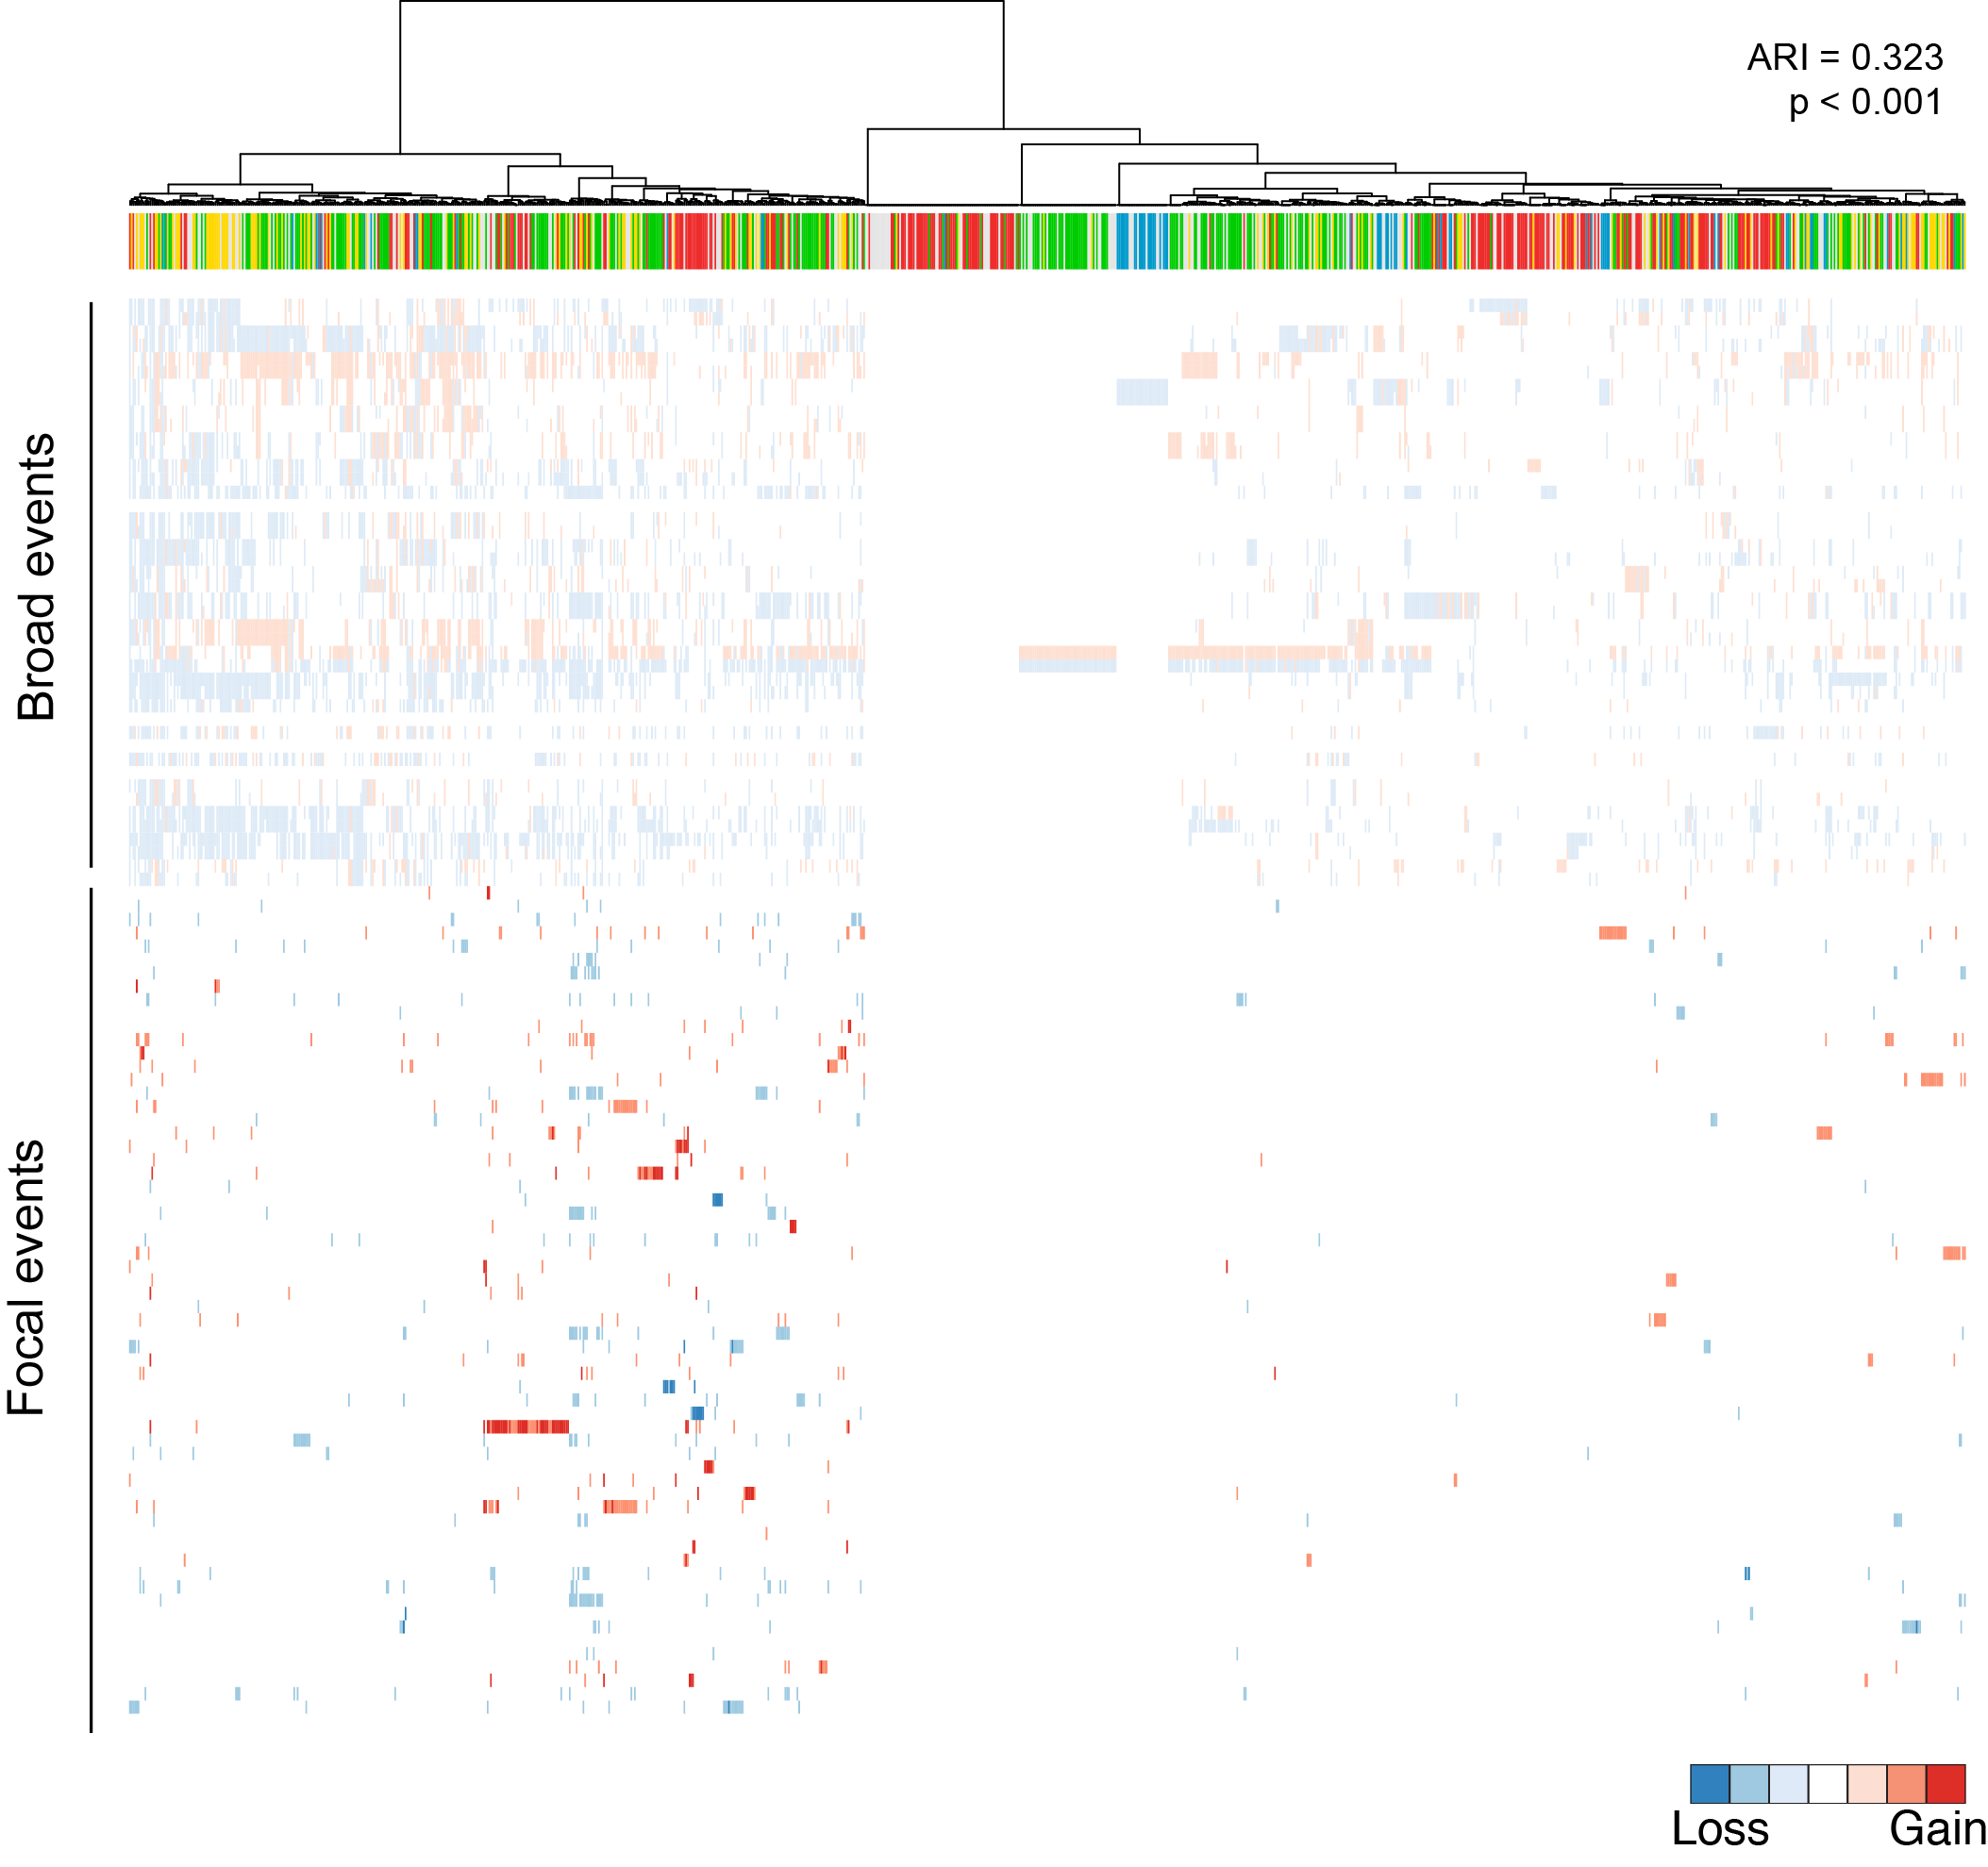
\includegraphics[width=\textwidth]{fig/magic-cn/cn-clusters.png}
	\end{center}
	\caption[Hierarchical clustering of broad and focal SCNAs in medulloblastoma]
	{
		Hierarchical clustering of broad and focal SCNAs in medulloblastoma.
		Agglomerative hierarchical clustering was performed on 827 primary medulloblastoma samples with known molecular subgroups, in order to assess the association between the clusters driven by DNA copy-number profiles and the classes defined by expression signatures. Coloured top-side bar indicates known expression subgroups (WNT: blue, SHH: red, Group~3: yellow, Group~4: green). Only focal events identified in the pan-cohort GISTIC2 analysis were included in the clustering. Resulting clusters show significant agreement with known expression subgroups ($p < 0.001$, $\chi^2$ test, $ARI = 0.323$). Adjusted Rand index ($ARI$) is a measure in $[0, 1]$ of the effect size of the agreement. 
	}
	\label{fig:cn-clusters}
\end{figure}

\clearpage

\section{Discussion}

This study raised several bioinformatic challenges particularly due to the lack of germline samples. Owing to current and historical practices, the medulloblastoma samples amassed in this study were often not paired with germline samples. Fortunately, somatic and germline copy-number events are distinguishable on account of the rarity of large germline copy-number variants (spanning $> 1$ Mbp or $> 10$ probes) in the control population \citeself{shih12}. Additionally, we also dismissed copy-number variants observed in both cases and controls at high frequency ($> 90$\%). Identified germline copy-number variants were removed from copy-number profiles along with the breakpoints they introduced. However, despite our best efforts, some likely germline events and hybridization artifacts (unrelated to submission batch but possibly related to reagent lot) remain in the copy-number profiles of the samples. Nonetheless, with additional post-processing, careful curation, focus on high frequency events, and integration with multiple sources of evidence, we successfully identified recurrently disrupted genomic loci, though we caution against the isolated use of individual tumour copy-number profiles for future studies. The poor interpretability of individual copy-number events in a single tumour sample stems from non-systematic hybridization biases, poor sample DNA quality, the general genomic instability of some samples, and the notion that most genetic events during cancer evolution do not contribute to cancer cell survival and tumour formation. In light of these limitations, we prioritized genomic events observed frequently across multiple samples. Furthermore, we split samples into more homogeneous groups in order to identify such events above a background mutation rate. Indeed, we discovered significantly more recurrent \gls{cna} when the samples were split by subgroup than when they were analyzed together, reinforcing the utility of classifying medulloblastoma as four distinct diseases. To emphasize, we discovered patterns hidden in complex genomic profiles of tumours by comparing and contrasting biologically similar groups of samples.

Another common issue that arises in cancer genomics studies is the role that genomic instability plays in tumour formation, progression, or recurrence. We contend that genomic instability in itself does not impact outcome, though the underlying cause or the consequent disruption of specific genes may affect tumour aggressiveness. For example, \gene{TP53} mutation may predispose to chromothripsis, but only the former portends poor outcome in multivariate survival analyses \citeref{shih14}. Chromothripsis does not exclusively occur in \gene{TP53} mutated cases; instead, it may be associated with mutations in other DNA damage response or repair genes, not all of which may contribute to tumour resistance against chemotherapy or radiotherapy. Further, chromothripsis in SHH medulloblastoma often results in amplification of \gene{GLI2}, but only the latter is independently prognostic for poor survival \citeref{shih14}. These findings in our medulloblastoma cohort contrast the association of chromothripsis with poorer survival (by univariate instead of multivariate analysis) in neuroblastoma \citeref{molenaar12}. Further, our pattern of chromothripsis incidence also contrasts that of a smaller cohort of medulloblastoma \citeref{rausch12}, in which the authors observed significantly higher frequency of chromothripsis in SHH medulloblastoma. In contrast, the incidence of chromothripsis is fairly uniform across SHH, Group3, and Group4 medulloblastomas and significantly depleted in WNT medulloblastoma. These results could be due to characteristic differences between the two cohorts of medulloblastoma examined. Both studies used the same method and algorithm to identify chromothripsis (the same researcher processed the raw SNP array data and made the chromothripsis calls in both studies). Interactions among competing covariates may obscure meaningful interpretation and may explain the observed discrepancies across studies; furthermore, recall biases in retrospective studies may skew distributions of specific variables, especially in studies with small sample sizes.

Notwithstanding the technical, biological, and statistical challenges, we have successfully identified recurrent amplifications and deletions of genes that converge on specific signaling pathways contributing to tumourigenesis within each molecular subgroup of medulloblastoma. WNT medulloblastoma is surprisingly devoid of recurrent genomic aberrations aside from chr6 loss and \gene{CTNNB1} activating mutation. While the functional consequence of chr6 is unclear, the high frequency of \gene{CTNNB1} mutation suggest that activated \gls{wnt} signaling may be the predominant tumourigenic mechanism in WNT medulloblastoma. Similarly, recurrent \gls{cna} events converge on and conspire to activate \gls{shh} signaling in SHH medulloblastoma. In a subset of SHH cases, TP53 signaling and \gls{pi3k} signaling are also recurrently disrupted by \gls{cna}, and the latter may be a candidate pathway for therapeutic intervention against tumours with aberrations upstream of the drug target. The dominant theme in Group3 medulloblastoma is recurrent disruption of signaling of the super \gls{tgfb} family; in particular, \gls{cna} converge on activation of activin signaling, and this pathway may be the first rational candidate pathway for therapeutic intervention in this aggressive subgroup. While no signaling pathway is highly recurrently dysregulated in Group4 medulloblastoma, tandem duplications of \gene{SNCAIP} is frequently observed and may play an important role in the pathogenesis of Group4 medulloblastoma. Taken together, copy-number profiling of medulloblastoma samples have led to the discovery of several frequently disrupted genes and pathways that may serve as candidates for targeted therapeutic intervention.

The disparate patterns of recurrent \gls{cna} among medulloblastoma subgroups not only support the distinct etiologies of the subgroups but also raise questions regarding the origin of the molecular subgroups of medulloblastoma. Most recurrent \gls{cna} were enriched (observed at higher frequency) in specific subgroups but were not exclusively found in one subgroup. Further, unsupervised clustering by copy-number profiles produced groups that showed only modest agreement with the molecular subgroups of medulloblastoma based on transcriptional profiles (\citefig{cn-clusters}). These results taken together suggest that the \gls{cna} events do not determine the molecular subgroups, though they may modulate the expression patterns of the subgroups. In contrast, DNA methylation patterns can identify, without supervision, four medulloblastoma classes that show high concordance with the subgroups identified by expression patterns \citeref{hovestadt13, schwalbe13}. This finding indicates that the epigenetic landscape in the cell of origin controls the expression patterns of the developing tumour and may also provide contexts that favours specific genomic aberrations, thus forming disparate genetic landscapes for each medulloblastoma subgroup.

The Myc family of proto-oncogenes is amplified in a curious pattern across the medulloblastoma subgroups, and this pattern poses a question regarding whether and how epigenetic patterns influence amplification patterns of the Myc family, comprising \gene{MYC}, \gene{MYCN}, and \gene{MYCL}. These homologous genes were found to be amplified in lymphoma, neuroblastoma, and lung carcinoma, respectively, which possibly points to functional differences in Myc family proteins in diverse cancer types. Similarly, Myc family genes are amplified in a non-random pattern in medulloblastoma: \gene{MYC} is amplified predominately (albeit not exclusively) in Group3, \gene{MYCN} is amplified preferentially in SHH and Group4 medulloblastomas, and rare \gene{MYCL} amplifications are observed only in SHH medulloblastoma. At the expression level, most medulloblastomas of either WNT or Group3 subgroup upregulate RNA expression of MYC independent of DNA amplification. Similarly, SHH medulloblastomas express MYCN at a higher level than other subgroups and normal cerebellums even without \gene{MYCN} amplification. 
In neuroblastoma, \gene{MYCN} amplification is found in about 20\% of cases \citeref{brodeur84, molenaar12}, but amplification of \gene{MYC} or \gene{MYCL} is very rarely observed \citeref{molenaar12}. These observations raise the question of why \gene{MYC}, \gene{MYCN}, and \gene{MYCL} is preferentially dysregulated in one cancer type or subtype as compared to another. Conceivably, Myc family genes could interact with different sets of co-transcription factors, drive dissimilar transcriptional programs, and cooperate with dysregulation of disparate signaling pathways in promoting tumour formation. Accordingly, the amplification of different Myc family genes could modulate the expression patterns of medulloblastoma subgroups. Additionally, genes nearby the \gene{MYC} or \gene{MYCN} locus can modulate the effect of amplifications spanning these loci.

An alternative hypothesis is that differential accessibilities at genomic loci in the cell of origin govern which of the three human Myc family gene is amplified. Under this model, \gene{MYCN} amplification preferentially occurs in SHH medulloblastoma because \gene{MYCN} is expressed in the cell of origin for SHH medulloblastoma (e.g. external granule neural precursor) during normal development, rendering the genomic locus accessible to such enzymes as deaminases (e.g. \gene{AICDA}, \gene{APOBEC}), which initiate double-strand breaks that can ultimately lead to DNA rearrangement. Similarly, \gene{MYC} amplification may preferentially occur in Group3 medulloblastoma because the \gene{MYC} locus is permissible to structural rearrangement in the cell of origin of Group3. In other words, the observed patterns of Myc family gene amplification can arise due to variations in accessibility of these genomic loci in different cellular origins instead of functional differences among Myc family members. Consistent with this model, MYCN is functionally redundant with MYC, and knock-in of \gene{MYCN} into the \gene{MYC} locus rescues the loss of \gene{MYC} in mouse development, cell growth, and cell differentiation \citeref{malynn00}. \gene{MYC} and \gene{MYCN} double knock-out mice exhibit much more severe phenotype in neurogenesis than either one alone, suggesting that loss of one Myc family member can be partially rescued by another member with overlapping expression pattern \citeref{wey10}. Further, \gene{MYC} and \gene{MYCN} are interchangeable in promoting tumour formation: \gene{MYCN} coding region can substitute for that of \gene{MYC} in the transformation of pro-B cell \citeref{gostissa09}. Similarly, MYC can cooperate with SHH ligand to enhance formation of SHH medulloblastoma in a virus-induced mouse tumour model, despite that \gene{MYC} amplification is rarely observed in human SHH medulloblastoma \citeref{rao03, shih12}. Therefore, Myc family genes may indeed encode functionally similar proteins (whose transcriptional regulation may differ) that promote medulloblastoma formation by a common mechanism.

Despite being an important player in transforming normal cells into cancer or in inducing pluripotency in differentiated cells, a Myc family gene may exert different effects in different tumour contexts. In Group3 medulloblastoma, \gene{MYC} amplification is associated with poorer survival. However, \gene{MYCN} amplification is associated with poorer survival only in SHH medulloblastoma but not in Group4 medulloblastoma \citeself{shih14}. The amplification of a Myc family gene is thus not universally associated with poorer outcome, and the function of Myc in medulloblastoma may be modulated by cooperating disruption of other pathways in the tumour-initiating cell and by extracellular signals in the context of neural development.

The story of the Myc family illustrates a broader theme of how genomic alterations lead to different subgroups of medulloblastoma. \gene{MYC} amplifications can drive tumour formation, but only in the suitable cellular context and with other cooperating mutations \citeref{rao03, pei12}. Indeed, \gene{MYC} and \gene{SHH} overexpression are sufficient to induce tumour formation in the external granule layer of the cerebellum but not in the cerebrum \citeref{rao03}. Accordingly, MYC overexpression alone likely does not create Group3 medulloblastoma. Rather, (possibly multiple) cellular origins and cooperating alterations provide the necessary context for the amplification of \gene{MYC} and consequent induction of medulloblastoma, and they dictate the molecular subgroup identity of the resulting tumour. Similarly, \gene{MYCN} amplification is a common mechanism of tumourigenesis in subsets of SHH and Group4 medulloblastoma cases, and this genetic event does not induce an overwhelming transcriptional change that by itself justifies the definition of an distinct \gene{MYCN}-amplified molecular subgroup. Indeed, gene amplification of the Myc family does not create a transcriptionally homogeneous entity that is distinct from other molecular subgroups. The functional outcome of Myc amplification very much depends on the molecular subgroup of the tumour in which Myc amplification occurs \citeself{shih14}. In experimental models, Myc family overexpression, along with cooperating mutations, can likely transform multiple cells of origin, and the subgroup of the resulting tumour would likely be determined by the cellular origin rather than the Myc family member. More generally, tumours of specific subtypes arise due to interaction between genetics and context. The cellular origin provides the permissive context for genomic alterations to exert their effects, and the nuclear organization, epigenetic landscape, chromatin architecture within the cell of origin jointly influence the accessibility of genomic loci and shape the mutational landscape of the cancer cell \citeref{polak15}.

In summary, medulloblastoma subgroups are characterized by distinct genomic alterations that disrupt disparate signaling pathways. The mutational profiles do not define each subgroup; instead, they are shaped by the molecular and cellular context within each subgroup, and the functional consequences of the mutations may also depend on the molecular subgroup. Hence, genes and pathways that are recurrently disrupted by genomic alterations within each subgroup likely play pivotal roles in the formation and perhaps maintenance of the tumours, and such genes and pathways serve as prime candidates for design of rational, targeted therapeutic intervention.
